\section{Optimal Path Planning Policy}
\label{sec:algorithm}

\subsection{Properties of Euler Trail}

Although the DFS-based approach is time-efficient, it has \emph{no} guarantee to minimize the number of generated paths, which will increase the telemetry overhead, especially the telemetry workload at the centralized controller (as mentioned in \S\ref{subsec:challenge}). Besides, it exerts no optimization on the balanced path generation. Here, we propose an optimal path planning algorithm taking advantage of the mathematical properties of the Euler trail/circuit. In graph theory, a trail is a walk in a graph (\eg, $v_0$, $e_1$, $v_1$, $e_2$, ..., $v_k$) without repeated edges and an Euler trail is a trail which visits every edge exactly once. Similarly, an Euler circuit is a special Euler trail which starts and ends on the same vertex. To clarify the important theorems of the Euler trail/circuit, we give the definition of \emph{odd vertex} first. An odd vertex is a vertex who has an odd degree (\eg, vertex 1, 3, 5, 6 in Fig.~\ref{fig:euler}(a)). The following four theorems are well proved in graph theory: (1) a connected graph with \emph{no} odd vertex has an Euler circuit; (2) a connected graph with only \emph{one} odd vertex does not exist; (3) a connected graph with \emph{two} odd vertices has an Euler trail starts from one odd vertex and ends at the other one; (4) a connected graph with \emph{2k} odd vertices contains at least $k$ distinct trails which, together, traverse all edges of the graph exactly once~\cite{bondy1976graph}. The proposed optimal algorithm heavily relies on the above theorems.

\subsection{Algorithm Description}

In fact, the above properties (especially theorem (4)) give the \emph{theoretical} value of the minimum non-overlapped path number for covering a given graph. \emph{To achieve the theoretical minimum, each extracted path from a graph should starts from an odd vertex and ends at another odd vertex.} In other words, removing one such path from a graph will eliminate a pair of odd vertices of that graph. According to the above observation, we devise an Euler-trail based algorithm to iteratively extract a path between a pair of odd vertices until all the vertices are extracted from the graph (\ie, the degree of every vertex becomes zero). For a given graph with $2k$ odd vertices, our algorithm will generate $k$ non-overlapped paths (the theoretical minimum) to cover all edges of the graph. 



Although the algorithm sounds rather straightforward as an iterative path extraction process, \emph{the devil lies in the detail} of dealing with multiple boundary cases. To be more specific, the devil lies in the possibility that an extracted path can split one connected graph into multiple subgraphs, which definitely complicates the iterative path extraction process. For example, from Fig.~\ref{fig:euler}(a) to Fig.~\ref{fig:euler}(b) after the extraction of path 1-4-3, the connected graph is split into two subgraphs. Besides, the algorithm also need deal with (sub)graphs with no odd vertex (\eg, subgraph \{1,2,3\} in Fig.~\ref{fig:euler}(b)). We put the pseudocode of the optimal algorithm in Fig.~\ref{fig:algorithm2} and explain it in detail. 

\begin{figure}
\centering
\epsfig{file=figure/algorithm2.eps, scale=0.64}
\vspace{-0.35cm}
\caption{Euler trail-based path planning algorithm.}
\label{fig:algorithm2}
\vspace{-0.44cm}
\end{figure} 

Actually, without considering the complexity of graph split, for a given connected graph, there are mainly three different cases for path extraction. If the graph contains two odd vertices, we just find an Euler trail between the two odd vertices as the path to be extracted. If the graph contains more than two odd vertices, we should extract an Euler trail between any pair of odd vertices. If the graph does not contain any odd vertex, we can extract an Euler circuit from the graph, which traverses every vertex of the graph.

Specifically, we use $G$ to represent the graph set, which is initialized to be one connected graph and will contain one connected graph or multiple subgraphs caused by path extraction. We use $Q$ to represent the path set which is initialized as an empty set and will finally contain the generated non-overlapped INT paths. We use $G-p$ to represent extracting a path $p$ from the graph set $G$ which will possibly further split the graph(s) into more subgraphs. First, we consider a simple case that the algorithm input contains only one connected graph. If the graph has no odd vertex, an Euler circuit can be found with the Hierholzer's algorithm~\cite{hierholzer1873moglichkeit} and inserted into $Q$ (as implemented in line 17-19 in Fig.~\ref{fig:algorithm2}). Here, the Hierholzer's algorithm is an algorithm for finding Euler trails/circuits with a run-time complexity of $O(E)$~\cite{fleischner1991x}, which is more efficient than the famous Fleury's algorithm~\cite{fleury1883deux}. If the graph has two odd vertices, an Euler trail can also be found with the Hierholzer's algorithm and inserted into $Q$ (line 25-26, line 31-32). If the graph has more than two odd vertices, we just randomly choose two odd vertices and find a path (\eg, with the Dijkstra's algorithm or any other algorithms) to connect the pair of odd vertices, then we insert the path into $Q$ (line 28-29, line 31-32). Notice that each time we extract a path from $G$ and insert it into $Q$, the graph(s) in $G$ may be broken into multiple disconnected subgraphs. Next, we discuss how to handle this boundary case in detail.

We use $S$ to save the disconnected subgraphs split from $G$ via DFS traversal (line 2). Then, we select graphs with \emph{no} odd vertex from $S$ and save them into $T$ (line 3). For each graph in set $T$, we can generate an Euler circuit $T\_circuit$ for its full edge coverage (line 9 and line 17). However, $T\_circuit$ is \emph{inadequate} to become a final INT path, since if the initial graph has $2k$ odd vertices ($k>0$), all the $k$ INT paths should connect $k$ pairs of odd vertices. By contrast, $T\_circuit$ does not contain any odd vertex. For this situation, there is only one possibility that $T\_circuit$ must be an integral part of a final INT path. In other words, $T\_circuit$ should be successfully connected to one calculated Euler trail to form a longer Euler trail. Here, we give a simple proof of the above hypothesis that $T\_circuit$ is an integral part of a final INT path.

\textbf{Proposition 1.}
In the Euler trail-based path planning algorithm (Fig.~\ref{fig:algorithm2}), if $T \neq \emptyset$ and $Q \neq \emptyset$ (\ie, there is at least one (sub)graph $g$ that does not contain odd vertex and there has been at least one calculated Euler trail in $Q$), $T\_circuit$ (the Euler circuit of $g$) should be successfully connected to one of the calculated Euler trails in $Q$ to form a longer Euler trail.

\begin{proof}
We construct a simple proof by \emph{contradiction}. Suppose $T\_circuit$ cannot connect to any of the Euler trails in $Q$. Then, there must be two possibilities: (1) $g$ itself is the initial graph $G$; (2) $g$ is once a part of the initial graph $G$. For case (1), if $g$ is the initial graph, then $Q$ must be an empty set, which contradicts with the premise that $Q \neq \emptyset$. For case (2), if $g$ is once a part of the initial graph $G$, then $g$ must have at least one common vertex $v$ with graph $G - T\_circuit$. If $T\_circuit$ cannot connect to any of the Euler trails in $Q$, then $v$ does not belong to any of the Euler trails in $Q$. However, according to the algorithm in Fig.~\ref{fig:algorithm2}, graph split occurs only after the extraction of Euler trails. If $v$ is not on the Euler trails, then $g$ must be still connected with $G - T\_circuit$ on $v$, which contradicts with the premise that $g$ is a separate subgraph.
\end{proof}

% 如果T_circuit无法连接Q中的欧拉路径,那么顶点v也无法连接Q中的欧拉路径。同时,根据我们的算法,图只能被产生的欧拉路径进行分割,如果v没有在欧拉路径上,那么T_circuit在算法运行完成后仍然和G-T_circuit相连,这就和T_circuit是一个独立的图相矛盾。


If $T \neq \emptyset$ and $Q \neq \emptyset$, we search the current $Q$ to find a path $T\_path$ having at least a same vertex with $T\_circuit$ (line 7). Then, we connect $T\_circuit$ with $T\_path$ to create a longer new path via \texttt{pathPaste()} (line 10) and replace the original $T\_path$ with the new path in $Q$ (line 8, 11).

In summary, the algorithm iteratively extracts paths connecting two odd vertices or pastes Euler circuits to the previous extracted paths to form the final INT paths. The algorithm halts if all the vertices are extracted from the graph (\ie, $G = \emptyset$).





\subsection{Case Study}
Fig.~\ref{fig:euler} exemplifies a path extraction process of the Euler trail-based algorithm. At the start, there is only one graph $G_1$ \{1,2,3,4,5,6,7\} with 4 odd vertices. Since the number of the odd vertices is larger than 2 (line 28), we randomly choose two odd vertices (1 and 3), extract a path 1-4-3 from $G_1$ and insert the path into $Q$ (Fig.~\ref{fig:euler}(a)). The above path extraction behavior will split the original $G_1$ into two subgraphs $G_1$ \{1,2,3\} and $G_2$ \{4,5,6,7\}. Since $G_1$ has no odd vertex and $Q \neq \emptyset$ (line 4-5), we paste the path 1-4-3 in $Q$ with the Euler circuit 1-2-3-1 generated from $G_1$ to create a new path 1-2-3-1-4-3. The new path will replace the original path 1-4-3 in $Q$ (Fig.~\ref{fig:euler}(b)). After the path paste, there is only one graph $G_1$ \{4,5,6,7\} with 2 odd vertices (line 25). We use the Hierholzer's algorithm to find its Euler trail 5-4-6-5-7-6 as the second INT path in $Q$ (Fig.~\ref{fig:euler}(c)). The algorithm halts since all the paths are extracted.

\subsection{Run-Time Complexity Analysis}
\label{subsec:theory}

The complexity of the above algorithm is analyzed. Since the algorithm is quite sophisticated, here, we strive to give an \emph{upper bound} for its run-time complexity as follows.

\textbf{Assumption.}
The input of the algorithm is an undirected connected graph $G=(V,E)$ with $2k$ odd vertices ($k = 0,1,2,...$). The graph is implemented via the adjacency list. We only consider the most time-consuming subprocedures in the algorithm, namely, (a) DFS for graph split (line 2), (b) \texttt{eulerCircuit()} and \texttt{eulerTrail()}, both using the Hierholzer's algorithm (line 9, 17, 26), (c) \texttt{randomTrail()} using the Dijkstra's algorithm (line 29). The time cost $T$ of the three subprocedures can be represented as $T(DFS(V,E)) = (E+V)t_0$, $T(Euler(V,E)) = Et_0$, $T(Dij(V,E)) = Et_0$, all based on their fastest implementation~\cite{cormen2009introduction, hierholzer1873moglichkeit, thorup1999undirected}, where $t_0$ is the one memory access time of the adjacency list.

\textbf{Complexity analysis case by case.}

1. If $k = 0,1$, $G$ has one Euler circuit or one Euler trail. In this case, DFS will be performed to check the graph connectivity, and \texttt{eulerCircuit()} or \texttt{eulerTrail()} will be performed to extract the path. Hence, the time cost can be derived as $T = T(DFS(V,E)) + T(Euler(V,E))$.

2. If $k > 1$, $G$ must have at least 4 odd vertices.

2.1. For the first iteration of the algorithm, DFS will be performed to check the connectivity, then, \texttt{randomTrail()} will be performed to extract one shortest path between 2 odd vertices. The time cost $T_1 = T(DFS(V,E)) + T(Dij(V,E))$.

2.2. For the next iteration, after the path extraction, the graph $G = (V, E)$ becomes $G' = (v, e)$. Then, we use DFS to check its connectivity. The path extraction may split $G'$ into subgraphs. We use $S$ to represent the subgraph set. For this step, the time cost $T_2 = T(DFS(v,e))$.

2.3. Set $S$ can further be partitioned into two subsets with one subset $T$ containing subgraphs \emph{without} odd vertices and the other subset $S-T$ containing subgraphs \emph{with} odd vertices. We define $T = \{g_x'|g_x'=(v_x', e_x'), x = 1,2,...\}$, $S-T = \{g_y''|g_y''=(v_y'',e_y''), y=1,2,...\}$. We have $\sum_{x}v_x' + \sum_{y}v_y'' = v$, $\sum_{x}e_x' + \sum_{y}e_y'' = e$.

2.4. For each subgraph $g_x'$ in subset $T$, we will perform \texttt{eulerCircuit()} and \texttt{pathPaste()}. Since \texttt{eulerCircuit()} is much more time-consuming, we only consider its time cost as $T_3 = \sum_xT(Euler(v_x',e_x'))$.

2.5. For each subgraph $g_y''$ in subset $S-T$, if $g_y''$ has exactly 2 odd vertices, we will perform \texttt{eulerTrail()}; if $g_y''$ has more than 2 odd vertices, we will perform \texttt{randomTrail()}. Given we have $y_1$ subgraphs with exactly 2 odd vertices and $y_2$ subgraphs with more than 2 odd vertices, the time cost of this step can be derived as $T_4 = \sum_{y_1}T(Euler(v_{y_1}'',e_{y_1}'')) + \sum_{y_2}T(Dij(v_{y_2}'',e_{y_2}''))$.

2.6. The iteration will go back to 2.2. until $G$ becomes $\emptyset$.

Given the algorithm is iterated for $m$ times, the total time cost can be derived as $T = T_1 + \sum_{i}^{m-1}(T_{2i} + T_{3i} + T_{4i})$, where $i$ stands for the ($i+1$)th iteration ($0 < i < m$).


\textbf{Upper bound derivation.}
The complexity of the algorithm lies in that the number of subgraphs in $T$ or $S-T$ for each iteration as well as the algorithm execution path cannot be predetermined. Here, we derive an \emph{upper bound} for algorithm's run-time complexity considering its \emph{worst-case execution path}. 

First, we try to solve $T_3 = \sum_xT(Euler(v_x',e_x'))$. Considering $T(Euler(v,e)) = et_0$, given $e' = \sum_{x}e_x'$, we have $T_3 = \sum_xT(Euler(v_x',e_x')) = \sum_{x}e_x't_0 = e't_0$.

Then, we try to solve $T_4$. According to our algorithm, the number of odd vertices of each subgraph in $S-T$ will be decreased by 2 in each iteration. Hence, the total number of decreased odd vertices in each iteration will be $2(y_1+y_2)$. According to the assumption, the total number of decreased odd vertices in $m$ iterations is $2k$. In the worst case, the iteration times $m$ should be \emph{maximized} while the number of decreased odd vertices in each iteration should be \emph{minimized}. In this case, $m = k$, $y_1 = 0, y_2 = 1$ for the first k-1 iterations and $y_1 = 1, y_2 = 0$ for the $k$th iteration. That is to say, the total number of decreased odd vertices in each iteration will be limited to 2. In this case, we have $T_{4i} = T(Dij(v_i'',e_i''))$ ($i = 1,2,...,k-2$) and $T_{4i} = T(Euler(v_i'',e_i''))$ ($i = k-1$).

According to the above analysis, we have $T = T_1 + \sum_{i}^{m-1}(T_{2i} + T_{3i} + T_{4i}) \le T(DFS(V,E)) + T(Dij(V,E)) + \sum_{i=1}^{k-2}(T(DFS(v_i,e_i)) + e_i't_0 + T(Dij(v_i'', e_i''))) + T(DFS(v_{k-1}, e_{k-1})) + e_{k-1}'t_0 + T(Euler(v_{k-1}'',e_{k-1}''))$, where $e_i$ is the edge set of $G' = (v,e)$,  $e_i'$ is the edge set of the subgraph subset $T$ and $e_i''$ is the edge set of the subgraph subset $S-T$, all in the ($i+1$)th iteration. Similarly, $v_i$ and $v_i''$ are the vertex sets of $G'$ and $S-T$, respectively. Apparently, we have $e_i = e_i' + e_i''$ and $v_i = v_i' + v_i''$.

According to the worst-case assumption, there is at least one subgraph in $T$ and there is only one subgraph in $S-T$ for each iteration. Therefore, $G_i'$ for the ($i+1$)th iteration is generated from $G_{i-1}'$ by removing all the subgraphs from $T$ and one shortest path from $S-T$. Using the above \emph{recurrence relation}, we can further derive algorithm's run-time complexity $T$. 

Actually, the minimal subgraph without odd vertices is the \emph{triangle}, which has 3 vertices and 3 edges, while the minimal shortest path is the \emph{line segment} which has 2 (odd) vertices and 1 edge. Therefore we have $e_i' \ge 3$, $v_i' \ge 3$, $e_i'' \ge 1$, $v_i'' \ge 2$, $e_i \le e_{i-1}-3-1$, $v_i \le v_{i-1} -3$. By plugging the initial values $e_0 = E, v_0 = V$ into the above relations, we have $e_i \le E-4i$, $v_i \le V - 3i$. Based on above relations, we can further derive

$e_i' = e_i - e_i'' \le e_i - 1 \le E-4i-1$,

$v_i' = v_i - v_i'' \le v_i - 2 \le V-3i-2$,

$e_i'' = e_i - e_i' \le e_i - 3 \le E-4i-3$,

$v_i'' = v_i - v_i' \le v_i - 3 \le V-3i-3$.

By plugging the above relations into the expression of $T$, we derive an upper bound for the run-time complexity as

$T \le (E+V)t_0 + Et_0 + \sum_{i=1}^{k-2}((e_i + v_i)t_0 + e_i't_0 + e_i''t_0) + (e_{k-1} + v_{k-1})t_0 + e_{k-1}'t_0 + e_{k-1}''t_0 \le (2E+V)t_0 + \sum_{i=1}^{k-1}(e_i + v_i + e_i' + e_i'')t_0 \le (2E+V)t_0 + \sum_{i=1}^{k-1}(E-4i + V-3i + E -4i -1 +E -4i -3)t_0 \le (3kE + kV - \frac{15}{2}k^2 -E + \frac{7}{2}k + 4)t_0$.

Therefore, one upper bound for algorithm's run-time complexity can be represented as $O(k(3E + V -\frac{15}{2}k))$.








\subsection{Heuristic for Balanced Path Generation}
\label{subsec:balance}

As mentioned in \S\ref{subsec:challenge}, balanced path generation is preferable to facilitate synchronized multi-path monitoring. However, our algorithm does not explicitly optimize for this particular purpose. Here, we propose a simple \emph{heuristic} for more balanced path generation based on the original algorithm. 

According to our extensive debugging of the original algorithm, we find that the path connecting two odd vertices generated by function \texttt{eulerTrail()} in line 26 is often \emph{too short} compared with the average length of the Euler trails. The reason lies in that in our implementation of \texttt{eulerTrail()}, we return the shortest path between two \emph{randomly} selected odd vertices with the Dijkstra's algorithm. If the path cannot properly paste to an Euler circuit afterwards to form a longer Euler trail, the final INT paths will be less balanced.

To address this issue, we propose a heuristic for more balanced path generation simply by rewriting the function \texttt{eulerTrail()}. Instead of returning the shortest path between two randomly selected odd vertices, we calculate all the shortest paths between any given pair of odd vertices and return the \emph{longest} path from all these shortest paths. Such a tweak greatly reduces the length variance of final INT paths.

However, on each extraction of an Euler trail, we have to recalculate $C_n^2$ ($n$ is the number of odd vertices) shortest paths due to the graph update, which is time-consuming. Here, we propose a technique to further minimize the computation cost. Actually, in our algorithm, we always remove edges from the graph during path extraction while never add edges into the graph. Hence, if the calculated shortest path has no intersection with the extracted Euler trail, the shortest path need not be recalculated. By checking the intersection of the extracted path and the shortest paths, we can update the shortest paths \emph{on demand} and eliminate unnecessary computation cost.





